\documentclass{article}
\usepackage[english,russian]{babel}
\usepackage{textcomp}
\usepackage{geometry}
  \geometry{left=2cm}
  \geometry{right=1.5cm}
  \geometry{top=1.5cm}
  \geometry{bottom=2cm}
\usepackage{tikz}
\usepackage{multicol}
\usepackage{listings}
\usepackage{amsthm}
\pagenumbering{gobble}

\lstdefinestyle{csMiptCppStyle}{
  language=C++,
  basicstyle=\linespread{1.1}\ttfamily,
  columns=fixed,
  fontadjust=true,
  basewidth=0.5em,
  keywordstyle=\color{blue}\bfseries,
  commentstyle=\color{gray},
  texcl=true,
  stringstyle=\ttfamily\color{orange!50!black},
  showstringspaces=false,
  %numbers=false,
  numbersep=5pt,
  numberstyle=\tiny\color{black},
  numberfirstline=true,
  stepnumber=1,      
  numbersep=10pt,
  backgroundcolor=\color{white},
  showstringspaces=false,
  captionpos=b,
  breaklines=true
  breakatwhitespace=true,
  xleftmargin=.2in,
  extendedchars=\true,
  keepspaces = true,
  tabsize=4,
  upquote=true,
}
\lstdefinestyle{csMiptCppBorderStyle}{
  style=csMiptCppStyle,
  framexleftmargin=5mm, 
  frame=shadowbox, 
  rulesepcolor=\color{gray}
}

\lstset{style=csMiptCppStyle}
\lstset{literate={~}{{\raisebox{0.5ex}{\texttildelow}}}{1}}
\begin{document}

\title{Семинар \#2: Классы и перегрузка операторов. \vspace{-5ex}}\date{}\maketitle
\section*{Классы}

\noindent \textbf{Объектно-ориентированное программирование (ООП)} -- это парадигма разработки программного обеспечения, основанная на использовании объектов, которые представляют собой экземпляры классов.\\

\noindent \textbf{Класс} -- это пользовательский тип данных, который объединяет данные и методы. Классы в C++ объявляются с помощью ключевого слова \texttt{struct} или с помощью ключевого слова \texttt{class}. \\

\noindent \textbf{Поля класса} -- это переменные, которые объявлены внутри класса.\\

\noindent \textbf{Методы класса} -- это функции, которые определены внутри класса и могут оперировать с его полями.\\

\noindent \textbf{Члены класса} -- это сущности, которые определены внутри класса. Поля класса и методы класса являются членами класса.\\

\noindent \textbf{Свободные функции} -- это функции, которые не являются методами, то есть просто обычные функции.\\

\noindent Рассмотрим пример простого класса \texttt{Book}:
\begin{lstlisting}
#include <iostream>
#include <string>

struct Book 
{
    std::string title;
    int price;

    void makeDiscount(int discount) 
    {
        if (price > discount)
            price -= discount;
        else
            price = 0;
    }
};

int main() 
{
    Book a = {"Harry Potter", 500};
    a.makeDiscount(100);
    std::cout << a.price << std::endl;  // Напечатает 400
}
\end{lstlisting}
Данный класс обладает двумя полями (\texttt{title} и \texttt{price}) и одним методом (\texttt{makeDiscount}). В отличии от структур языка C, классы языка C++ могут содержать внутри себя функции, называемые методами. В функции \texttt{main} был создан объект класса \texttt{Book}, под названием \texttt{a}. Вызов метода у объекта осуществляется через специальный оператор точка:
\begin{lstlisting}
a.makeDiscount(100);
\end{lstlisting}
Внутри метода \texttt{makeDiscount} можно пользоваться полями класса. И если мы вызываем метод от объекта \texttt{a}, то будут использоваться поля объекта \texttt{a}.

\newpage
\subsection*{Инкапсуляция}
\noindent \textbf{Инкапсуляция} -- это размещение в классе полей и функций, которые работают с этими полями. Рассмотрим два разных класса \texttt{Book}. Первый класс не будет включать функцию для работы с его полями; такая функцию будут находиться вне класса. Это подход, при котором класс используется без инкапсуляции. Второй класс, напротив, будет применять инкапсуляцию, и функции для работы с его полями будут реализованы внутри класса.
\begin{multicols}{2}\setlength{\columnseprule}{0.4pt}
\textbf{Без инкапсуляции:}
\begin{lstlisting}
#include <iostream>
#include <string>

struct Book 
{
    std::string title;
    int price;
};

void makeDiscount(Book& b, int discount) 
{
	if (b.price > discount)
		b.price -= discount;
	else
		b.price = 0;
}

int main() 
{
    Book a = {"Harry Potter", 500};
    makeDiscount(a, 100);
    std::cout << a.price << std::endl;
}
\end{lstlisting}

\textbf{С инкапсуляцией:}
\begin{lstlisting}
#include <iostream>
#include <string>

struct Book 
{
    std::string title;
    int price;

    void makeDiscount(int discount) 
    {
        if (price > discount)
            price -= discount;
        else
            price = 0;
    }
};

int main() 
{
    Book a = {"Harry Potter", 500};
    a.makeDiscount(100);
    std::cout << a.price << std::endl;
}
\end{lstlisting}
\end{multicols}


\subsection*{Константные методы класса}
\noindent \textbf{Константный метод класса} -- это метод, который не может изменить поля объекта, на котором он вызывается. Константные методы помечаются словом \texttt{const} при объявлении метода класса. Например, в следующем примере класс \texttt{Book} имеет константный метод \texttt{printTitle}:\\
\begin{lstlisting}
struct Book 
{
    std::string title;
    int price;

    void printTitle() const 
    {
        std::cout << title << std::endl;
    }
};
\end{lstlisting}
Внутри класса \texttt{printTitle} нельзя изменять методы \texttt{title} и \texttt{price}. Попытка изменить поля внутри константного метода приведет к ошибке компиляции. Очень важно всегда указывать то, что метод является константным, если внутри него поля не изменяются.


\newpage


\section*{Скрытие данных}
\subsection*{Модификаторы доступа \texttt{public} и \texttt{private}}
Модификаторы доступа служат для ограничения доступа к полям и методам класса.
\begin{itemize}
\item \texttt{public} -- поля и методы могут использоваться где угодно
\item \texttt{private} -- поля и методы могут использовать только методы этого класса и друзья (особые функции и классы, объявленные с использованием ключевого слова \texttt{friend})
\end{itemize}
Создадим класс под название \texttt{Alice}, который будет содержать приватное поле \texttt{x}, приватный метод \texttt{cat}, публичное поле \texttt{y} и публичный метод \texttt{dog}. Попытаемся использовать эти члены класса из другого метода класса и вне этого класса. Внутри класса можно использовать любые члены класса, а вне класса можно использовать только публичные члены класса.
\begin{lstlisting}
#include <iostream>
#include <string>

struct Alice 
{
private:
    int x;
    void cat() const 
    {
    	std::cout << "cat" << std::endl;
    }
    
public:
	int y;
	void dog() const 
	{
		std::cout << "dog" << std::endl;
	}
	
	void test()
	{
		x = 10;  // OK, приватные поля можно использовать в самом классе
		cat();   // OK, приватные методы можно использовать в самом классе
		
		y = 10;  // OK, публичные поля можно использовать где угодно
		dog();   // OK, публичные методы можно использовать где угодно
	}
};

int main() 
{
    Alice a;
    
    a.x = 10;  // Ошибка, нельзя использовать приватные поля вне класса
    a.fx();    // Ошибка, нельзя использовать приватные методы вне класса
    
    a.y = 20;  // OK, поле y публичное
    a.dog();   // OK, метод dog публичный
    a.test();  // ОК, метод test публичный
}
\end{lstlisting}




\subsection*{Друзья}
\noindent \textbf{Друзья класса} -- это такие функции или классы, которые имеют доступ к приватным членам класса. Для обозначения того, что функция или класс является дружественной, используется ключевое слово \texttt{friend}:\\
В следующем примере был создан класс \texttt{Alice} у которого есть два друга: функция \texttt{func} и класс \texttt{Bob}. Мы можем вызывать приватный метод \texttt{cat} класса \texttt{Alice} из функции \texttt{func} и класса \texttt{Bob}, так как это друзья класса \texttt{Alice}.
\begin{lstlisting}
#include <iostream>
struct Alice 
{
private:
    void cat() const {std::cout << "cat" << std::endl;}
public:
    friend void func();  // Указываем, что функция func является другом класса Alice
    friend struct Bob;   // Указываем, что класс Bob является другом класса Alice
};

void func()
{
    Alice a;
    a.cat();  // Несмотря на то, что метод cat приватный, функция func имеет к нему доступ
}

struct Bob 
{
    void test()
    {
        Alice a;
        a.cat();  // Несмотря на то, что метод cat приватный, класс Bob имеет к нему доступ
    }
};

int main() 
{
    func();
    Bob b;
    b.test();
}
\end{lstlisting}
Дружественность не является симметричной. Если один класс является другом второго, то это не означает, что второй класс является другом первого. Например, в примере выше, \texttt{Bob} является другом \texttt{Alice}, но \texttt{Alice} не является другом \texttt{Bob}, поэтому \texttt{Alice} не имеет доступа к приватным полям и методам класса \texttt{Bob}.


\subsection*{Различие между определение класса с помощью \texttt{class} и \texttt{struct}}
Классы в языке C++ можно создавать как с помощью ключевого слова \texttt{struct}, так и с помощью ключевого слова \texttt{class}. Есть ровно два отличия между этими двумя вариантами определения классов.
Первое различие заключается в том, что у классов, созданных с использованием \texttt{struct}, все члены по умолчанию публичны, в то время как у классов, созданных с помощью \texttt{class}, члены по умолчанию являются приватными. Второе различие мы пройдём позже.
\begin{multicols}{2}\noindent
\begin{lstlisting}
struct Alice
{
	int x; // Это публичное поле
};
\end{lstlisting}

\begin{lstlisting}
class Alice
{
	int x; // Это приватное поле
};
\end{lstlisting} 
\end{multicols}


\newpage
\section*{Конструкторы и деструкторы}
Конструктор -- это метод класса, который вызывается автоматически при создании объекта класса. Конструкторы используются для инициализации объектов классов. Для того, чтобы создать конструктор, нужно в классе прописать метод без возвращаемого значение и с именем, совпадающим с названием класса. Перепишем класс \texttt{Book} из прошлых примеров так, чтобы его поля были приватными, но у класса был бы конструктор, который бы задавал эти поля:
\begin{lstlisting}
#include <iostream>
#include <string>

class Book 
{
private:
    std::string title;
    int price;
    
public:
	Book(const std::string& x, int y)
	{
		std::cout << "Constructor" << std::endl;
		title = x;
		price = y;
	}

    void print() const
    {
        std::cout << title << " " << price << std::endl;
    }
};

int main() 
{
    Book b("Dune", 500);  // Напечатает Constructor
    b.print();			  // Напечатает Dune 500
}
\end{lstlisting}
В данном примере нельзя задать значения полей объекта вне класса, так как они приватные. Но можно вызвать конструктор, который будет инициализировать эти поля. В строке:
\begin{lstlisting}
Book b("Dune", 500);
\end{lstlisting}
создаётся объект \texttt{a} типа \texttt{Book}. При создания этого объекта и вызывается написанный нами конструктор, который задаёт поля соответствующими значениями.

\subsection*{Различные синтаксисы вызова конструктора}
Язык C++ обладает богатой историей, в течение которой в него были добавлены множество новых возможностей. В результате, многие задачи в C++ можно решать различными способами. В частности, существует как минимум три способа создания объекта класса: с использование знака равенства, с использованием круглых скобок и с использованием фигурных скобок.
\begin{lstlisting}
Book a = {"Dune", 500}; // Похоже на инициализацию структуры из C, но вызовется конструктор
Book b("Dune", 500);    // Изначальный синтаксис C++.
Book c{"Dune", 500};    // Синтаксис, введённый в стандарте C++11.
\end{lstlisting}
Все эти способы делают одно и то же, а именно, создают объект класса с вызовом конструктора этого класса.\\
\newpage

\subsection*{Перегрузка конструкторов}
Как и другие функции и методы, конструкторы можно перегружать. В этом примере создадим у класса \texttt{Book} два конструктора. Первый конструктор будет иметь один параметр -- цену книги, а название книги этот конструктор будет задавать значением \texttt{"Harry Potter"}. Второй конструктор будет, как и раньше, иметь два параметра.
\begin{lstlisting}
#include <iostream>
#include <string>

class Book 
{
private:
    std::string title;
    int price;
    
public:
	Book(int y)
	{
		std::cout << "One" << std::endl;
		title = "Harry Potter";
		price = y;
	}

	Book(const std::string& x, int y)
	{
		std::cout << "Two" << std::endl;
		title = x;
		price = y;
	}

    void print() const
    {
        std::cout << title << " " << price << std::endl;
    }
};

int main() 
{
	Book a = {100};          // Напечатает One, способ вызова через символ =
	Book b = 100;            // Напечатает One, способ вызова через символ =
	Book c(100);             // Напечатает One, способ вызова через круглые скобки
	Book d{100};             // Напечатает One, способ вызова через фигурные скобки
	a.print();				 // Напечатает Harry Potter 100

    Book e = {"Dune", 500};  // Напечатает Two, способ вызова через символ =
    Book f("Dune", 500);     // Напечатает Two, способ вызова через круглые скобки
    Book g{"Dune", 500};     // Напечатает Two, способ вызова через фигурные скобки
	e.print();				 // Напечатает Dune 500
}
\end{lstlisting}
В функции \texttt{main} были созданы объекты класса \texttt{Book} различными способами, используя два разных конструктора. Обратите внимание, что если у конструктора один параметр, то при использовании синтаксиса с знаком равенства, фигурные скобки можно опустить.

\newpage


\subsection*{Конструктор по умолчанию и конструктор копирования}
\noindent \textbf{Конструктор по умолчанию} (англ. \textit{default constructor}) -- это конструктор, который не принимает аргументов.\\

\noindent \textbf{Конструктор копирования} (англ. \textit{copy constructor}) -- это конструктор, который принимает по ссылке один аргумент такого же типа, что и данный класс.\\

\noindent Создадим класс с конструктором по умолчанию и конструктором копирования:
\begin{lstlisting}
#include <iostream>
#include <string>

class Book 
{
private:
    std::string title;
    int price;
    
public:
	Book()
	{
		std::cout << "Default" << std::endl;
		title = "Harry Potter";
		price = 1000;
	}
	
	Book(const Book& other)
	{
		std::cout << "Copy" << std::endl;
		title = other.title;
		price = other.price;
	}

    void print() const
    {
        std::cout << title << " " << price << std::endl;
    }
};

int main() 
{
	Book a;       // Напечатает Default, ещё один способ
	Book b = {};  // Напечатает Default, способ вызова через символ =
	Book c();     // Ошибка, такой способ не работает для конструктора по умолчанию, так как
				  // невозможно отличить от прототипа функции.
	Book d{};     // Напечатает Default, способ вызова через фигурные скобки
	a.print();    // Напечатает Harry Potter 1000
	
	Book e = a;   // Напечатает Copy, способ вызова через символ =
	Book f(a);    // Напечатает Copy, способ вызова через круглые скобки
	Book g{a};    // Напечатает Copy, способ вызова через фигурные скобки
	e.print();    // Напечатает Harry Potter 1000
}
\end{lstlisting}
\subsection*{Конструкторы и передача в функции/возврат из функций}
Конструкторы также вызываются при передаче в функции, которые принимают по значению, и при возврате из функций. В данном примере есть функция \texttt{cat}, которая принимает объект типа \texttt{Book} по значению. Можно передавать в эту функцию аргументы конструктора класса \texttt{Book} в фигурных скобках. В этом случае внутри функции будет создан объект с помощью соответствующего конструктора. Если у конструктора один параметр, то фигурные скобки можно опустить. Аналогичным образом всё работает при возврате из функции. 
\begin{lstlisting}
#include <iostream>
#include <string>

class Book 
{
private:
    std::string title;
    int price;
public:
	Book(int y)
	{
		std::cout << "One ";
		title = "Harry Potter";
		price = y;
	}
	Book(const std::string& x, int y)
	{
		std::cout << "Two ";
		title = x;
		price = y;
	}
    void print() const
    {
        std::cout << title << " " << price << std::endl;
    }
};

void cat(Book x)
{
	x.print();
}

Book dog()
{
	return {"Brave New World", 1000};
}

int main() 
{
	cat({"Dune", 500});  // Напечатает Two Dune 500
	cat({500});          // Напечатает One Harry Potter 500
	cat(500);            // Напечатает One Harry Potter 500
	
	Book b = dog();      // Напечатает Two
	b.print();           // Напечатает Brave New World 1000
}
\end{lstlisting}

\subsection*{Конструкторы копирования и передача в функции/возврат из функций}
Чаще всего в фунции передаются уже созданные объекты. Что если в функцию, которая принимает по значению, передать уж созданный объект? В этом случае работают такие же правила, что и прежде. Вызовется конструктор, который сможет принять объект такого типа, то есть вызовется конструктор копирования. Однако, в похожем случае при возврате из функции, конструктор копирования почему-то не вызывается...
\begin{lstlisting}
#include <iostream>
#include <string>
class Book 
{
private:
    std::string title;
    int price;
public:
    Book(const std::string& x, int y)
    {
        title = x;
        price = y;
    }
    
    Book(const Book& other)
    {
        std::cout << "Copy ";
        title = other.title;
        price = other.price;
    }
    
    void print() const
    {
        std::cout << title << " " << price << std::endl;
    }
};

void cat(Book x)
{
    x.print();
}

Book dog()
{
    Book b("Brave New World", 1000);
    return b;
}

int main() 
{
    Book a("Dune", 500);
    cat({a});        // Напечатает Copy Dune 500
    cat(a);          // Напечатает Copy Dune 500
    
    Book b = dog();  // НЕ напечатает Copy (почему? это более сложный вопрос)
    b.print();       // Напечатает Brave New World 1000
}
\end{lstlisting}


\newpage
\subsection*{Деструктор}
Деструктор -- это метод класса, который вызывается автоматически при уничтожении объекта класса. Для переменных в сегменте стек, это происходит при выходе из области видимости в которой находится объект. Название деструктора состоит из символа тильда ($\sim$) и названия класса. Деструктор не принимает никаких аргументов.
\begin{lstlisting}
#include <iostream>
#include <string>

class Book 
{
private:
    std::string title;
    int price;
public:
    Book(const std::string& x, int y)
    {
        title = x;
        price = y;
        std::cout << "Constructor " << title << std::endl;
    }
    
    ~Book()
    {
        std::cout << "Destructor  " << title << std::endl;
    }
};

int main() 
{
    Book a("Cat", 500);
    Book b("Dog", 1000);
    
    if (true)
    {
        Book c("Mouse", 2000);
    }
    std::cout << "End of main" << std::endl;
}
\end{lstlisting}
Данная программа напечатает:
\begin{verbatim}
    Constructor Cat
    Constructor Dog
    Constructor Mouse
    Destructor  Mouse
    End of main
    Destructor  Dog
    Destructor  Cat
\end{verbatim}
Порядок вызова деструкторов для объектов в одной области видимости является обратным к вызову конструкторов. Данный порядок вызова деструкторов имеет смысл, так как есть значительная вероятность, что объект созданный позже будет зависить от предыдущих объектов. Если бы деструкторы вызывались в другом порядке, и объекты созданные раньше удалялись бы раньше, то мы не смогли бы удалить следующие объекты, так как они бы зависили от уже удалённых объектов.

\newpage
\subsection*{RAII}
\noindent \textbf{RAII} (Resource Acquisition Is Initialization) -- это идиома программирования, которая обеспечивает управление ресурсами с помощью автоматического освобождения ресурсов при выходе из области видимости.\\

Дословное \textit{Resource Acquisition Is Initialization} можно перевести как \textit{Получение ресурса это инициализация}, хотя более точно эту идиому следовало бы назвать как \textit{Получение ресурса это инициализация, а освобождение ресурса это деинициализация}. Основной смысл этой идиомы заключается в том, что следует получать ресурс в конструкторах, а освобождать ресурс в деструкторах. Ресурсом в данном контексте чаще всего является память в куче, но может быть и нечто другое, например, файловый дескриптор или объект устанавливающий соединение по сети.

Приведём пример использования идиомы RAII. Предположим, что по какой-то причине мы не можем использовать \texttt{std::string} в классе \texttt{Book}, а вместо этого должны сами выделять память в куче, в которой будем хранить название книги. Выделять память будем в конструкторе, а освобождать память, очевидно, следует в деструкторе. Это и есть смысл идиомы RAII.
\begin{lstlisting}
#include <iostream>
#include <cstdlib>
#include <cstring>

class Book 
{
private:
    char* title;
    int price;
public:
    Book(const char* x, int y)
    {
        title = static_cast<char*>(std::malloc((strlen(x) + 1) * sizeof(char)));
        std::strcpy(title, x);
        price = y;
    }
    
    ~Book()
    {
        std::free(title);
    }
    
    void print() const
    {
        std::cout << title << std::endl;
    }
};

int main() 
{
    Book a("Dune", 500); // Память под строку "Dune"{} выделится в конструкторе
    					 // и освободится в деструкторе 
}
\end{lstlisting}
Таким образом, если мы будем использовать эту идиому, то память будет освобождаться автоматически при уничтожении объекта и нам больше не нужно будет думать о корректномы выделении и освобождении памяти. В C++ есть большое количество классов, которые используют эту идиому. Например, классы \texttt{std::string} и \texttt{std::vector} используют идиому RAII.


\subsection*{Указатель \texttt{this}}
\begin{lstlisting}
#include <iostream>
using std::cout, std::endl;

struct Book 
{
    char title[100];
    float price;
    int pages;

    void printThis() const
    {
        cout << this << endl;
    }

    void printTitle() const
    {
        cout << title << endl;
        cout << this->title << endl;
    }

    void setPrice(float price)
    {
        this->price = price;
    }
};

int main() 
{
    Book a = {"War and Peace", 1700, 900};
    cout << &a << endl;
    a.printThis();
    a.printTitle();
}

\end{lstlisting}

\subsection*{Геттеры и сеттеры}

\newpage
\section*{Перегрузка операторов}

\subsection*{Перегруженный оператор, как свободная функций}

\subsection*{Какие операторы можно перегружать}

\subsection*{Особенности перегрузки операторов сравнения}


\subsection*{Перегрузка оператора \texttt{<{}<} с объектом \texttt{std::ostream}}

\subsection*{Перегруженный оператор, как метод класса}

\subsection*{Перегруженный оператор присваивания}
Ключевое слово \texttt{this} - это указатель на экземпляр класса, который можно использовать в методах этого класса.\\
Оператор присваивания -- это просто перегруженный оператор \texttt{=}. Оператор присваивания должен вернуть ссылку на текущий объект, то есть \texttt{*this}.\\

Нужно различать оператор присваивания и вызов конструктора:
\begin{lstlisting}
Point a = Point(7, 3);  // Конструктор ( оператор присваивания не вызывается )
Point b = a;            // Конструктор копирования ( оператор присваивания не вызывается )
Point c;                // Конструктор по умолчанию
c = a;                  // Оператор присваивания
\end{lstlisting}
Оператор присваивания должен возвращать ссылку на левый аргумент.


\subsection*{Перегруженный оператор стрелка \texttt{->}}


\newpage
\section*{Создаём свой класс комплексного числа}
Используем полученные знания для создания класса комплесных чисел. В данной реализации комплексных чисел все перегруженные операторы являются свободными функциями, хотя большинство из них можно было бы сделать методами.
\begin{lstlisting}[style=csMiptCppBorderStyle]
#include <cmath>
#include <iostream>

namespace mipt {
struct Complex 
{
    float re;
    float im;
};

// Арифметические операторы, два комплексных числа
Complex operator+(Complex a, Complex b) 
{
    Complex result = {a.re + b.re, a.im + b.im};
    return result;
}

Complex operator-(Complex a, Complex b) 
{
    Complex result = {a.re - b.re, a.im - b.im};
    return result;
}

Complex operator*(Complex a, Complex b) 
{
    Complex result = {a.re * b.re - a.im * b.im, a.re * b.im + a.im * b.re};
    return result;
}

Complex operator/(Complex a, Complex b) 
{
    float bSquared = a.re * a.re + a.im * a.im;
   
    Complex result;
    result.re = (a.re * b.re + a.im * b.im) / bSquared;
    result.im = (a.im * b.re - a.re * b.im) / bSquared;
    return result;
}

// Арифметические операторы, комплексное число и вещественное
Complex operator+(Complex a, float b) 
{
    Complex result = {a.re + b, a.im};
    return result;
}



Complex operator+(float a, Complex b) 
{
    return b + a;
}

Complex operator-(Complex a, float b) 
{
    Complex result = {a.re - b, a.im};
    return result;
}

Complex operator-(float a, Complex b) 
{
    return b - a;
}

Complex operator*(Complex a, float b) 
{
    Complex result = {a.re * b, a.im * b};
    return result;
}

Complex operator*(float a, Complex b) 
{
    return b * a;
}

Complex operator/(Complex a, float b) 
{
    Complex result = {a.re / b, a.im / b};
    return result;
}

Complex operator/(float a, Complex b) 
{
    Complex ac = {a, 0.0f};
    return ac / b;
}

// Операторы присваиваний сложения и т. п.
Complex& operator+=(Complex& a, Complex b) 
{
    a.re += b.re;
    a.im += b.im;
    return a;
}
Complex& operator-=(Complex& a, Complex b) 
{
    a.re -= b.re;
    a.im -= b.im;
    return a;
}

Complex& operator+=(Complex& a, float b) 
{
    a.re += b;
    return a;
}
Complex& operator-=(Complex& a, float b) 
{
    a.re -= b;
    return a;
}

Complex& operator*=(Complex& a, float b) 
{
    a.re *= b;
    a.im *= b;
    return a;
}

Complex& operator/=(Complex& a, float b) 
{
    a.re /= b;
    a.im /= b;
    return a;
}


// Унарные операторы
Complex operator+(Complex a) 
{
    return a;
}

Complex operator-(Complex a) 
{
    Complex result;
    result.re = -a.re;
    result.im = -a.im;
    return result;
}

Complex operator*(Complex a) 
{
    Complex result = {};
    result.re =  a.re;
    result.im = -a.im;
    return result;
}





/*
    Перегружаем оператор<< между типами std::ostream (такой тип имеет std::cout) и Complex
    для удобного вывода комплексных чисел на экран.

    Обратите внимание, что мы возвращаем ссылку на ostream.
    Таким образом результатом выражения  cout << a  будет cout.
    Поэтому можно делать так: cout << a << b << c ...
*/

std::ostream& operator<<(std::ostream& out, Complex a) 
{
    if (a.re != 0)
        out << a.re;

    if (a.im > 0)
    {
        if (a.im != 1.0)
            out << " + " << a.im << "i";
        else
            out << " + i";
    }
    else if (a.im < 0) 
    {
        if (a.im != -1.0)
            out << " - " << -a.im << "i";
        else
            out << " - i";
    }
    return out;
}
// Перегружаем оператор >> с объектом типа std::istream (такой тип имеет std::cin)
std::istream& operator>>(std::istream& in, Complex& c) 
{
    in >> c.re >> c.im;
    return in;
}
}

int main()
{
	mipt::Complex a = {1, 2};
	mipt::Complex b = {3, -1};
	
	std::cout << a + b << std::endl;  // Напечатает 4 + i
	std::cout << a * b << std::endl;  // Напечатает 5 + 5i
	std::cout << a / b << std::endl;  // Напечатает 0.2 + 1.4i
}
\end{lstlisting}
\newpage
\section*{Создаём свой класс строки}
Строки в языке \texttt{C} представляют собой просто массивы с элементами типа \texttt{char}(однобайтовое число). Работать с такими строками не очень удобно. Нужно выделять и удалять необходимую память, следить за тем, чтобы строка помещалась в эту память на всём этапе выполнения программы, для работы со этими строками нужно использовать специальные функции из библиотеки \texttt{string.h}. Это всё может привести к ошибкам. В этом разделе мы создадим класс \texttt{String} -- класс строки, с которым удобнее и безопаснее работать, чем со строками в стиле \texttt{C}. Заготовка класса выглядит так (Это далеко не самая эффективная реализация строки, более правильная реализация создаётся в примерах кода):
\begin{lstlisting}
#include <cstdlib>

class String 
{
private:

    size_t size;
    char* data;
    
public:

    String(const char* str) 
    {
        size = 0;
        while (str[size])
            size++;
		
        data = (char*)malloc(sizeof(char) * (size + 1));
		
        for (int i = 0; str[i]; i++)
            data[i] = str[i];
        data[size] = '\0';
    }
	
    size_t getSize() const 
    {
        return size;
    }
    
    const char* cStr() const 
    {
        return data;
    }
};

int main() 
{
    String a = "Elephant";
}
\end{lstlisting}

Схематично это можно представить следующим образом:
\begin{center}
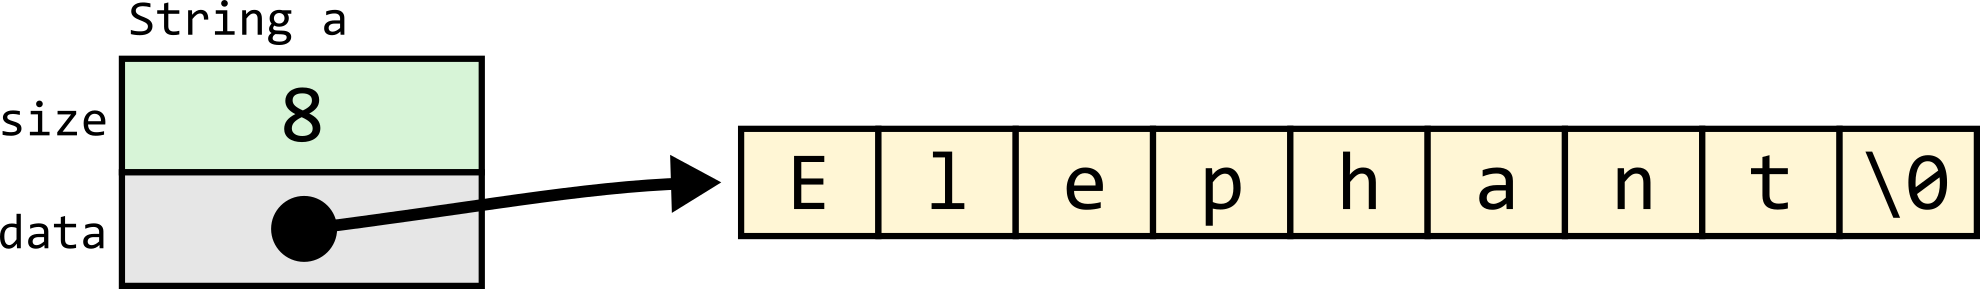
\includegraphics[scale=0.86]{../images/string_base.png}
\end{center}

\newpage

\section*{Особые методы класса}

\section*{Удалённые функции и \texttt{default}-функции}


\iffalse
\subsection*{Деструктор}
В коде выше выделяется память для массива \texttt{data}. Эта память выделяется при вызове конструктора (то есть при создании объекта). Однако она нигде не освобождается. Освободить её вручную мы не можем, так как поле \texttt{data} является приватным и это бы противоречило принципу сокрытия данных. Эта память должна освобождаться автоматически при удалении объекта.
\begin{lstlisting}
~ String() 
{
    free(data);
}
\end{lstlisting}

\subsection*{Перегруженные операторы класса \texttt{String}}
\begin{itemize}
\item \textbf{Оператор сложения:} \texttt{String operator+(const String\& right) const} \\
Этот оператор должен создавать новый экземпляр, задавать его поля (в частности придётся выделить память под строку-сумму) и возвращать этот экземпляр.

\item \textbf{Оператор присваивания сложения:} \texttt{String\& operator+=(const String\& right)}\\
Этот оператор не должен создавать новый экземпляр. Он должен изменять левый операнд (т. е. сам объект), и возвращать ссылку на этот объект (т. е. \texttt{*this}).

\item \textbf{Оператор присваивания:} \texttt{String\& operator=(const String\& right)}\\
Этот оператор не должен создавать новый экземпляр. Он должен изменять левый операнд (т. е. сам объект), так чтобы он стал идентичен правому. Если размеры строк не совпадают, то в данной реализации строки вам придётся удалить память левой строки и снова выделить память нужного размера. При этом нужно отдельно рассмотреть случай когда левый и правый операнд это один и тот же объект. 
\begin{lstlisting}
String a {"Cat"};
a = a;
\end{lstlisting}
Конечно, в этом случае ничего удалять не нужно.

\item \textbf{Оператор сравнения:} \texttt{bool operator==(const String\& right) const}\\
Этот оператор должен сравнивать строки (массивы \texttt{data}) и возвращать \texttt{true} или \texttt{false}.

\item \textbf{Оператор индексации:} \texttt{char\& operator[](unsigned int i)}\\
Этот оператор должен возвращать ссылку на \texttt{i}-ый символ строки.

\item \textbf{Индексация с проверкой на выход за границы:} \texttt{char\& at(unsigned int i)}\\
Этот метод должен проверять, что индекс \texttt{i} не выходит за границы диапазона и, если это так, возвращать ссылку на \texttt{i}-ый символ строки. Иначе, этот метод должен печатать сообщение об ошибке и завершать программу.
\end{itemize}
\fi

\newpage
\section*{Раздельная компиляция класса}
Методы можно вынести из определения класса следующим образом:
\begin{multicols}{2}\setlength{\columnseprule}{0.4pt}
\textbf{Определение методов в теле класса:}
\begin{lstlisting}
#include <cmath>
#include <iostream>


struct Point 
{
    float x, y;

    float norm() const 
    {
        return std::sqrt(x *x + y * y);
    }

    void normalize() 
    {
        float pnorm = norm();
        x /= pnorm;
        y /= pnorm;
    }

    Point operator+(const Point& r) const 
    {
        Point result = {x + r.x, y + r.y};
        return result;
    }
};





int main()
{
	Point p = {1, 2};
	p.normalize();
	std::cout << p.x << " " 
              << p.y << std::endl;
}
\end{lstlisting}
\vfill\null
\columnbreak

\textbf{Определение методов вне тела класса:}
\begin{lstlisting}
#include <cmath>
#include <iostream>

struct Point 
{
    float x, y;

    float norm() const;
    void normalize();
    Point operator+(const Point& r) const;
};

float Point::norm() const 
{
    return sqrt(x*x + y*y);
}

void Point::normalize() 
{
    float pnorm = norm();
    x /= pnorm;
    y /= pnorm;
}

Point Point::operator+(const Point& r) const
{
    Point result = {x + r.x, y + r.y};
    return result;
}

int main() 
{
	Point p = {1, 2};
	p.normalize();
	std::cout << p.x << " " 
              << p.y << std::endl;
}
\end{lstlisting}
\end{multicols}

Теперь эти методы можно скомпилировать отдельно. Для этого их нужно вынести в отдельный компилируемый файл \texttt{point.cpp}, а определение класса в отдельный файл \texttt{point.h}. Так называемый заголовочный файл \texttt{point.h} нужен, так как определение класса нужно и файле \texttt{point.cpp} и в файле \texttt{main.cpp}. Для компиляции используем:
\begin{verbatim}
g++ main.cpp point.cpp
\end{verbatim}

\begin{center}
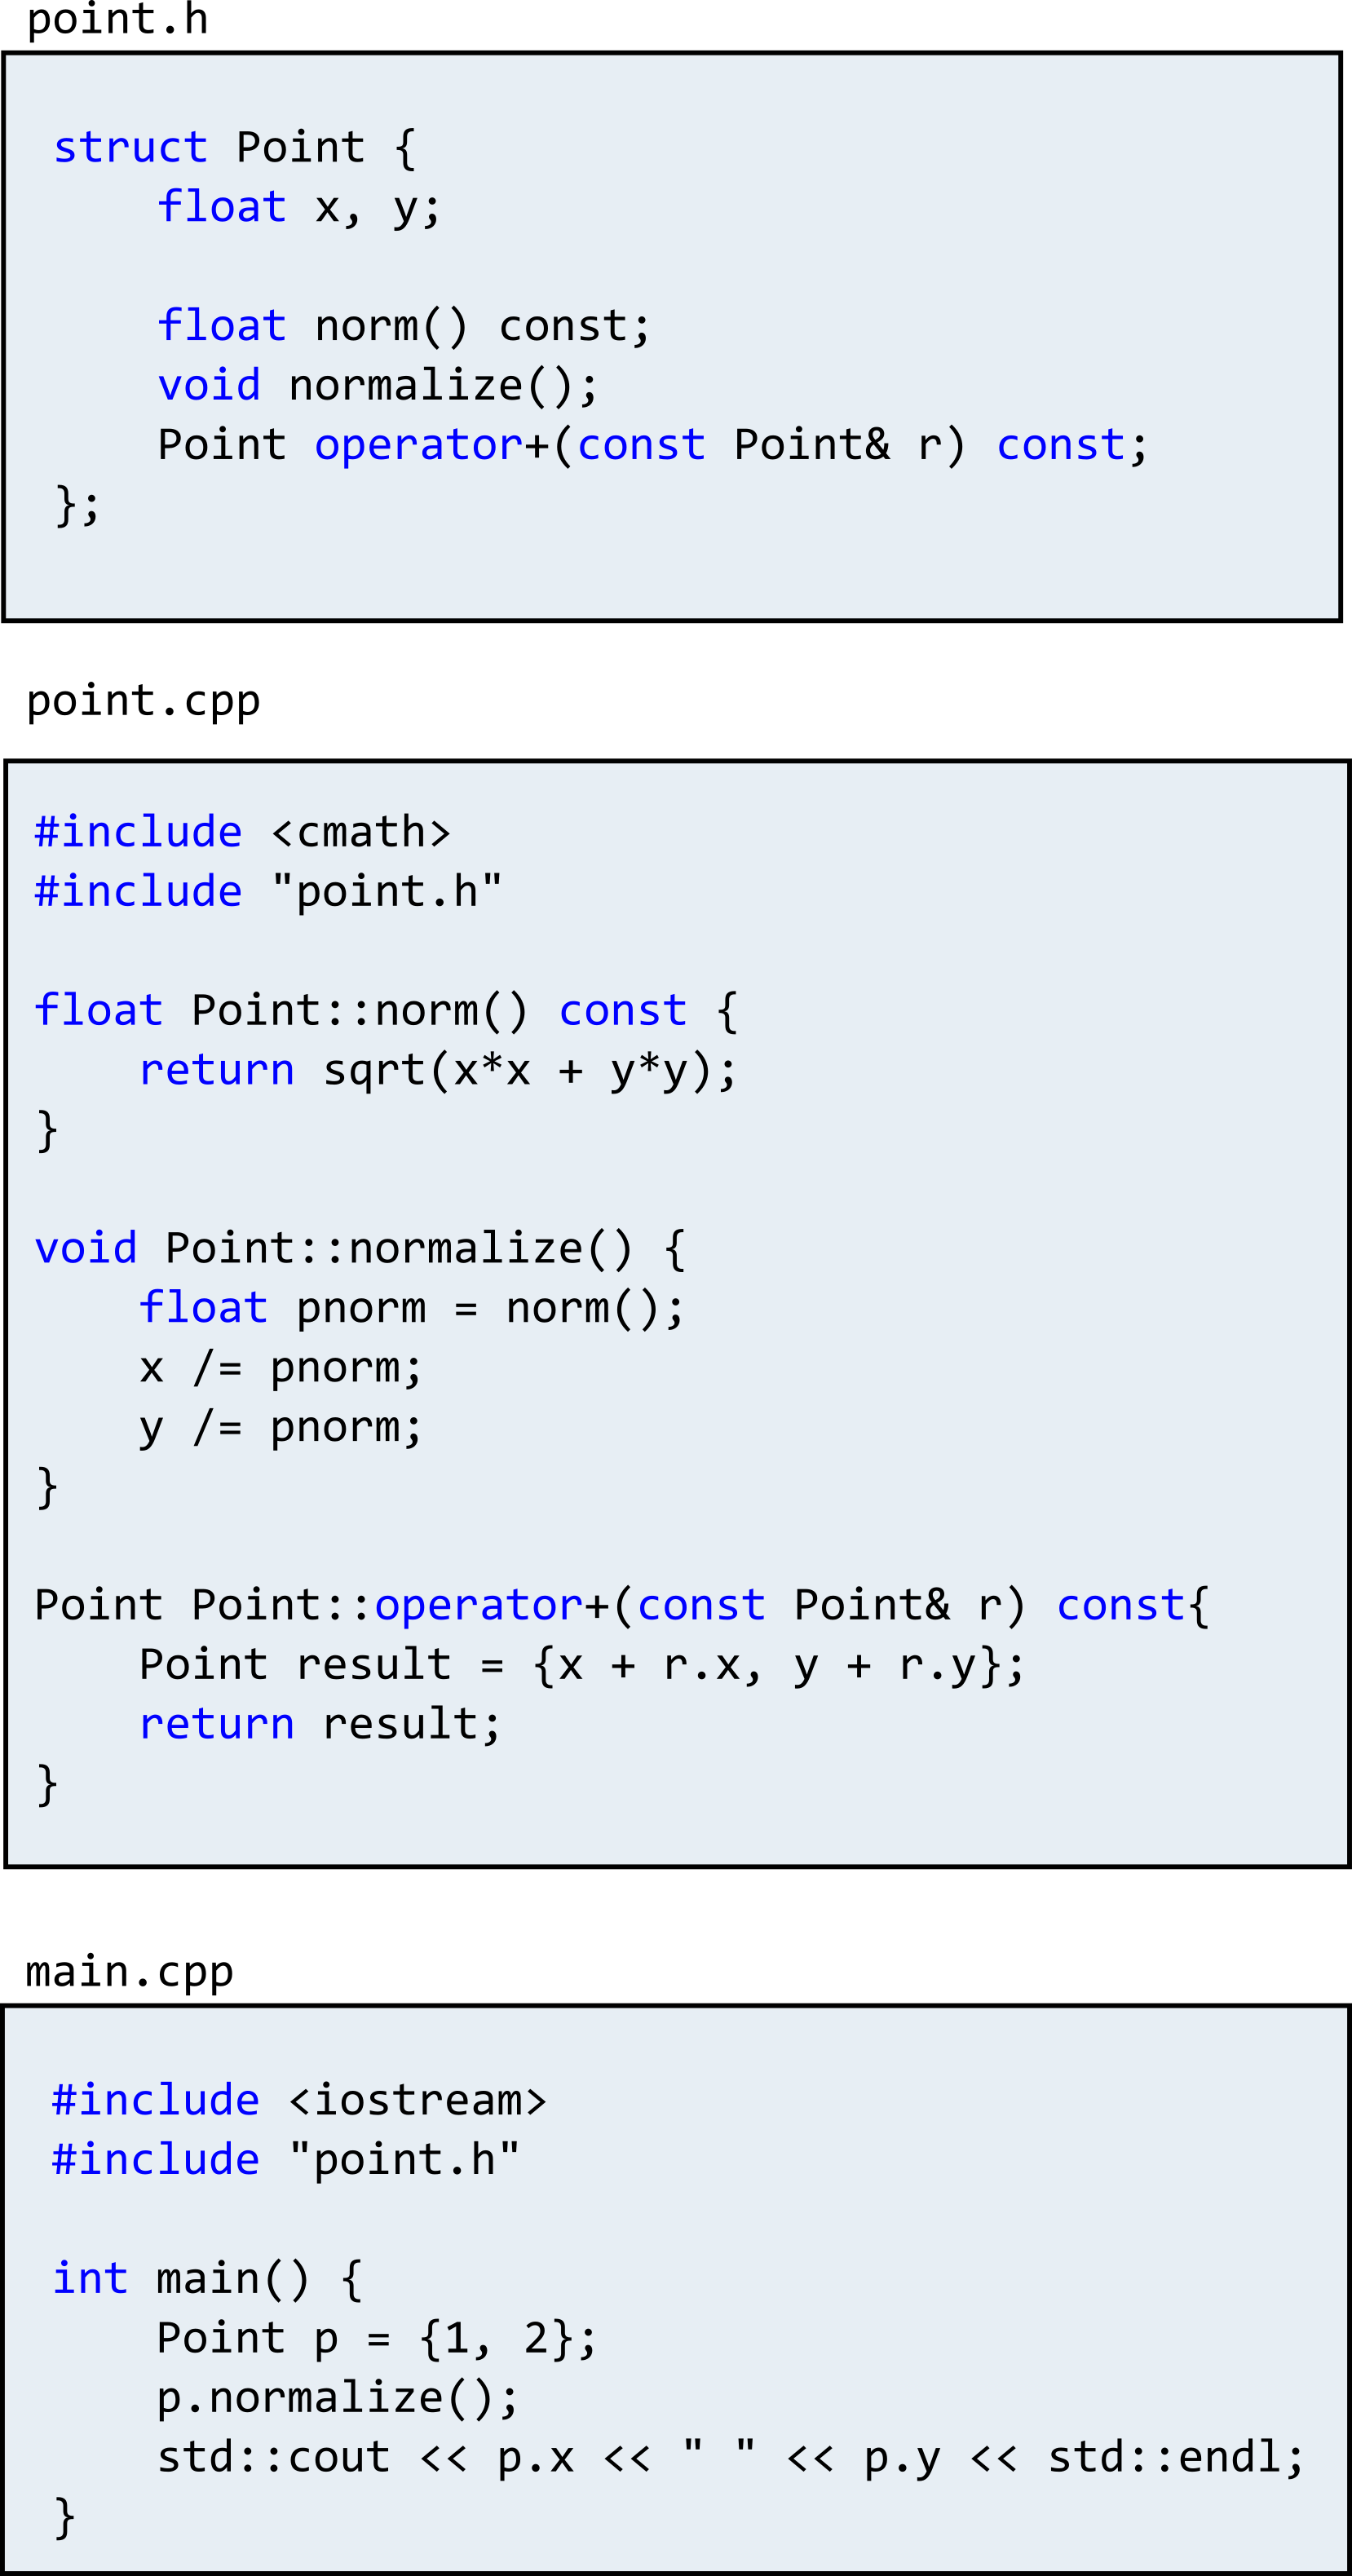
\includegraphics[scale=0.65]{../images/sepcompilation.png}
\end{center}

\end{document}
